\input{head.inc}
\usepackage{tikz-3dplot}
\usetikzlibrary{shapes.geometric}
\usepackage{pgfplots}
\pgfplotsset{compat = newest}
\newcommand{\Tube}[6][]%
% [further options], width, iterations, inner color, outer color, path definition
{   \colorlet{InColor}{#4}
    \colorlet{OutColor}{#5}
    \foreach \I in {1,...,#3}
    {   \pgfmathsetlengthmacro{\h}{(\I-1)/#3*#2}
        \pgfmathsetlengthmacro{\r}{sqrt(pow(#2,2)-pow(\h,2))}
        \pgfmathsetmacro{\c}{(\I-0.5)/#3*100}
        \draw[InColor!\c!OutColor, line width=\r, #1] #6;
    }
}

% Präambelbefehle für die Präsentation
\title[TET: Wellenleiter I - Zylindrische Wellenleiter]{TET: Wellenleiter I - Zylindrische Wellenleiter}

\begin{document}
% 
% Frontmatter 
% 
%%%%%%%%%%%%%%%%%%%%%%%%%%%%%%%%%%%%%%%%%%%%%%%%%%%%%%%%%%%%%%%%%%%%%%%%%%%%%%%%%%%%%%%%%%%%%%%%%%%%%%%%%%%%%%%%%%%%%%%%%%%%% 

%% inserts the title page and the table of contents
\maketitle

% 
% Content 
% 
%%%%%%%%%%%%%%%%%%%%%%%%%%%%%%%%%%%%%%%%%%%%%%%%%%%%%%%%%%%%%%%%%%%%%%%%%%%%%%%%%%%%%%%%%%%%%%%%%%%%%%%%%%%%%%%%%%%%%%%%%%%%% 
\section{TET: Wellenleiter I - Zylindrische Wellenleiter}

\begin{frame}
  \frametitle{Ausgangspunkt}
  \begin{itemize}[<+->]
  \item Viele Formen von \alert{Wellenleitern} in technischer Nutzung
  \item Beispiele:

    \begin{columns}[t]
      \begin{column}{.25\linewidth}
        Hohlleiter
\bigskip
        
      \def\r{1.8}			
\tdplotsetmaincoords{70}{120}
\begin{tikzpicture}[tdplot_main_coords]
  % Drawing XYZ coordinates system
  \def \lenX {1.0*\r}
  \def \lenY {1.0*\r}
  \def \lenZ {0.3*\r}
  \def \boxX{.7*\r}
  \def \boxY{.9*\r}
  \def \boxZ{.2*\r}
  % Calculate box corner length
  \pgfmathsetmacro{\boxCornerLen}{sqrt{((\boxX)^2 + (\boxY)^2 + (\boxZ)^2)}}
  % Draw coordinate system
  \draw[dashed] (0,0,0) -- (\boxX,0,0);
  \draw[-stealth,thin] (\boxX,0,0) -- (\lenX,0,0) node[left] {$y$};
  \draw[dashed] (0,0,0) -- (0,\boxY,0);
  \draw[-stealth,thin] (0,\boxY,0) -- (0,\lenY,0) node[anchor=north west] {$z$};
  \draw[dashed] (0,0,0) -- (0,0,\boxZ);
  \draw[-stealth,thin] (0,0,\boxZ) -- (0,0,\lenZ) node[anchor=south] {$x$};
  
  % Drawing horizontal box:
  % Get corner polar coordinate
  \tdplotgetpolarcoords{\boxX}{\boxY}{\boxZ}
  \tdplotsetcoord{Box}{\boxCornerLen}{\tdplotrestheta}{\tdplotresphi}
  % Draw a box
  \draw[] (Boxx) -- (Boxxy);
  \draw[very thick] (Boxy) -- (Boxxy);
  \draw[] (Boxx) -- (Boxxz);
  \draw[] (Boxz) -- (Boxxz);
  \draw[very thick] (Boxy) -- (Boxyz);
  \draw[] (Boxz) -- (Boxyz);
  \draw[very thick] (Boxxy) -- (Box);
  \draw[] (Boxxz) -- (Box);
  \draw[very thick] (Boxyz) -- (Box);
\end{tikzpicture}

\end{column}
      \begin{column}{.25\linewidth}
        Koaxialkabel
        
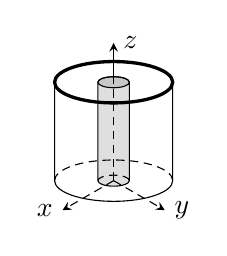
\begin{tikzpicture}
  \draw [fill=gray, fill opacity=.25] (180:2mm) coordinate (a) 
  -- ++(0,-12.5mm) coordinate (b)
  arc (180:360:2mm and .7mm) coordinate (d) % 2 war 5
  -- (a -| d) coordinate (c) arc (0:180:2mm and .7mm); % 2 war 5
  \draw [fill=gray, fill opacity=.25]
  (0,0) coordinate (t) circle (2mm and .7mm);
  \draw [densely dashed] (d) arc (0:180:2mm and .7mm);
  \draw []
  (180:7.5mm) coordinate (A)
  -- ++(0,-12.5mm) coordinate (B) 
  arc (180:360:7.5mm and 2.625mm) coordinate (D)
  -- (A -| D) coordinate (C) arc (0:180:7.5mm and 2.625mm);
  \draw [very thick]
  (0,0) coordinate (T) circle (7.5mm and 2.625mm);
  \draw [densely dashed] (D) arc (0:180:7.5mm and 2.625mm);
  \draw [densely dashed ]
  ([yshift=-12.5mm]T) coordinate (B)
  edge [-stealth] node [pos=1, right] {$y$} +(-30:7.5mm)
  edge [-stealth] node [pos=1, left] {$x$} +(-150:7.5mm)
  -- (T) edge [solid, -stealth] node [right, pos=1] {$z$} ++(0,5mm) ;
\end{tikzpicture}

\end{column}
\begin{column}{.25\linewidth}
  Zweidrahtleitung (Lecher-Leitung)

  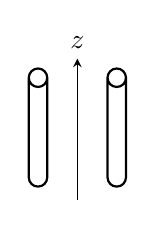
\begin{tikzpicture}
\node [thick,cylinder, draw, shape border rotate=90,minimum height=1.5cm,minimum width=2mm] at (0,0){}; 
\node [thick,cylinder, draw, shape border rotate=90,minimum height=1.5cm,minimum width=2mm] at (1cm,0cm){};
\draw[thin, -stealth] (0.5cm,-0.80cm) -- (0.5cm,1cm) node[above]{$z$};
\end{tikzpicture}

        \end{column}
        \begin{column}{.25\linewidth}
          Mikrostreifenleitung
\bigskip
          
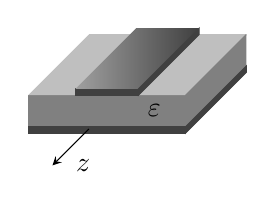
\begin{tikzpicture}[scale=0.4]
  \draw [lightgray] (0,1,0) coordinate (bl) -- (5,1,0) coordinate (br);
  \filldraw [gray] (0,0,5) coordinate (fll) -- (0,1,5) coordinate (ftl) -- (5,1,5) coordinate (ftr) -- (5,0,5) coordinate (flr) -- cycle;
  \shade [left color = lightgray, right color = lightgray] (bl) -- (br) -- (ftr) -- (ftl) -- cycle;
  \filldraw [gray] (5,0,0) coordinate (blr) -- (flr) -- (ftr) -- (br);
  \filldraw [darkgray] (fll) rectangle (5,-0.2,5) coordinate (flr2);
  \filldraw [darkgray] (flr2) -- (5,-0.2,0) coordinate (blr2) -- (blr) -- (flr) -- cycle;
  \filldraw [darkgray] (1.5,1.2,5) coordinate (ftl-1) -- (3.5,1.2,5) coordinate (ftr-1) -- (3.5,1,5) coordinate (flr-1) -- (1.5,1,5) coordinate (fll-1) -- cycle;
  \shade [left color = darkgray!50, right color = darkgray] (1.5,1.2,0) coordinate (btl-1) -- (3.5,1.2,0) coordinate (btr-1) -- (ftr-1) -- (ftl-1) -- cycle;
  \filldraw [darkgray] (flr-1) -- (ftr-1) -- (btr-1) --  (br -| btr-1) -- cycle;
  \node at (4,0.5,5) {$\varepsilon$};
  \coordinate (nA1) at (1.5,2.5,0);
  \coordinate (nB1) at (3.5,2.5,0);
  \coordinate (nA2) at (-1.5,1.2,0);
  \coordinate (nB2) at (-1.5,1.2,5);
  \coordinate (nA3) at (7,1,5);
  \coordinate (nB3) at (7,1.2,5);
  \coordinate (nA4) at (-1.5,1,5);
  \coordinate (nB4) at (-1.5,0,5);
  \draw[-stealth,thin] (0,-2,0) -- (0,-2,3) node[right,xshift=5]{$z$};
\end{tikzpicture}
          
        \end{column}
      \end{columns}
    \item Die Strukturen sind in $z$-Richtung \alert{translationsinvariant} \(\to\) Alle Schnitte senkrecht zu $z$ sind identisch!
    \item In diesem Fall sprechen wir von \alert{zylindrischen Wellenleitern}.
    \item Wir betrachten hier nur Wellenleiter mit metallischen Begrenzungen (als ideal leitend angenommen)
    \item Dielektrische Wellenleiter (\(\to\) Totalreflexion) werden hier nicht betrachtet.
      \item Zwei Betrachtungsweisen: Feldtheoretisch (geht immer) und (klassische) \alert{Leitungstheorie} (mit Strom und Spannung; geht teilweise \(\to\) später).
  \end{itemize}
  \end{frame}

\begin{frame}
  \frametitle{Zylindrische Wellenleiter}
  \begin{columns}
    \begin{column}{.3\linewidth}
  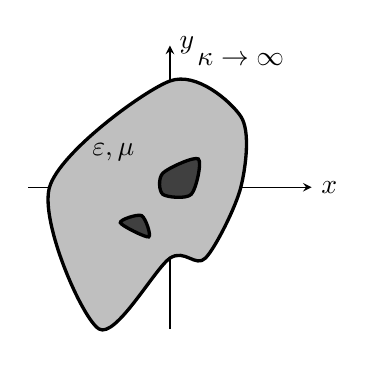
\begin{tikzpicture}[scale=.9]
    \draw [thin, -stealth] (-2,0) -- (2,0) node[right]{$x$};
    \draw [thin, -stealth] (0,-2) -- (0,2) node[right]{$y$};
    \draw [very thick, draw=black, fill=lightgray] plot [smooth cycle] coordinates {(-1,-2) (-1.7,0) (0,1.5) (1,1) (1,0) (0.5,-1) (0,-1)};
    \draw [very thick, fill=darkgray] plot [smooth cycle] coordinates {(-.7,-.5) (-.4,-.4) (-.3,-.7)}; 
    \draw [very thick, fill=darkgray] plot [smooth cycle] coordinates {(-.1,-.1) (-.1,.2) (0.4,0.4) (.3,-.1)}; 
    \node at (1,1.8){$\kappa\to\infty$}; 
    \node at (-.8,.5){$\varepsilon,\mu$}; 
  \end{tikzpicture}
  \end{column}
  \begin{column}{.7\linewidth}
      \begin{itemize}[<+->]
      \item Die Vektoren \(\einheitsvek{x}\) und \(\einheitsvek{y}\) spannen die \alert{Querschnittsebene} oder \alert{Transversalebene} auf.
      \item Voraussetzung: Alle Querschnittsebenen (für verschiedene \(z\)) sind identisch.
      \item Lösungsgebiet: lineares, homogenes, isotropes Dielektrikum mit \(\varepsilon, \mu\)
      \item Alles andere: perfekte Leiter (\(\kappa \to \infty\))
        \item Wir betrachten den Fall der \alert{harmonischen Zeitabhängigkeit}.
        \end{itemize}
  \end{column}
    \end{columns}
      \begin{itemize}[<+->]
      \item Homogene Wellengleichung (\(\frac{\d}{\d t}\)) \(\to\) \alert{Helmholtz-Gleichung} (\(\komplex\omega\))
        \begin{align*}
          \square \EFeld[uv](\Ortsr[v], t) = \left(\laplace - \varepsilon\mu\frac{\d^2}{\d t^2}\right) \EFeld[uv] (\Ortsr[v], t) = \vec{0} &&\rightarrow  &&\left(\laplace + \varepsilon\mu\omega^2\right) \EFeld[uv](\Ortsr[v]) =\vec{0} \\
          \square \BFeld[uv](\Ortsr[v], t) = \left(\laplace - \varepsilon\mu\frac{\d^2}{\d t^2}\right) \BFeld[uv] (\Ortsr[v], t) = \vec{0} &&\rightarrow  &&\left(\laplace + \varepsilon\mu\omega^2\right) \BFeld[uv](\Ortsr[v]) =\vec{0} 
        \end{align*}
        %\item Lösung in Zylinderkoordinaten \((\rho,\varphi,z)\)
        \end{itemize}
\end{frame}


\begin{frame}
  \frametitle{Zylinder-Geometrie -- Vektorzerlegung}
  \begin{columns}
    \begin{column}{.35\textwidth}
  % set the plot display orientation
%synatax: \tdplotsetdisplay{\theta_d}{\phi_d}
\tdplotsetmaincoords{60}{110}

%define polar coordinates for some vector
%TODO: look into using 3d spherical coordinate system
\pgfmathsetmacro{\rvec}{.5}
\pgfmathsetmacro{\thetavec}{30}
\pgfmathsetmacro{\phivec}{60}

%start tikz picture, and use the tdplot_main_coords style to implement the display 
%coordinate transformation provided by 3dplot
\begin{tikzpicture}[scale=5,tdplot_main_coords]

%set up some coordinates 
%-----------------------
\coordinate (O) at (0,0,0);

%determine a coordinate (P) using (r,\theta,\phi) coordinates.  This command
%also determines (Pxy), (Pxz), and (Pyz): the xy-, xz-, and yz-projections
%of the point (P).
%syntax: \tdplotsetcoord{Coordinate name without parentheses}{r}{\theta}{\phi}
\tdplotsetcoord{P}{\rvec}{\thetavec}{\phivec}

%draw figure contents
%--------------------

%draw the main coordinate system axes
\draw[thick,->] (0,0,0) -- (.5,0,0) node[anchor=north east]{$x$};
\draw[thick,->] (0,0,0) -- (0,.5,0) node[anchor=north west]{$y$};
\draw[thick,->] (0,0,0) -- (0,0,.5) node[anchor=south]{$z$};

%draw a vector from origin to point (P) 
\draw[-stealth,color=red,thick] (O) -- (P) node[midway, above,xshift=-5]{$\vec{E}$} node[above,black]{$(\textcolor{green}{x}, \textcolor{green}{y}, \textcolor{cyan}{z})$} ;
%\draw[-stealth,color=green,thick] (P) -- +(0,0,0.2) node[above]{$\VektorPot[uv]=\VektorPot[u]_z\einheitsvek{z}$};

%draw projection on xy plane, and a connecting line
\draw[color=green, -stealth] (O) -- (Pxy) node[right]{$\vec{E}_t$};
\draw[color=cyan, -stealth] (Pxy) -- (P) node[midway, right]{$\vec{E}_z$};

%draw the angle \phi, and label it
%syntax: \tdplotdrawarc[coordinate frame, draw options]{center point}{r}{angle}{label options}{label}
%\tdplotdrawarc{(O)}{0.1}{0}{\phivec}{anchor=north}{$\varphi$}


%set the rotated coordinate system so the x'-y' plane lies within the
%"theta plane" of the main coordinate system
%syntax: \tdplotsetthetaplanecoords{\phi}
\tdplotsetthetaplanecoords{\phivec}

%draw theta arc and label, using rotated coordinate system
%\tdplotdrawarc[tdplot_rotated_coords]{(0,0,0)}{0.3}{0}{\thetavec}{anchor=south west}{$\vartheta$}

%draw some dashed arcs, demonstrating direct arc drawing
%\draw[dashed,tdplot_rotated_coords] (\rvec,0,0) arc (0:90:\rvec);
%\draw[dashed] (\rvec,0,0) arc (0:90:\rvec);

%set the rotated coordinate definition within display using a translation
%coordinate and Euler angles in the "z(\alpha)y(\beta)z(\gamma)" euler rotation convention
%syntax: \tdplotsetrotatedcoords{\alpha}{\beta}{\gamma}
\tdplotsetrotatedcoords{\phivec}{\thetavec}{0}

%translate the rotated coordinate system
%syntax: \tdplotsetrotatedcoordsorigin{point}
\tdplotsetrotatedcoordsorigin{(P)}

%use the tdplot_rotated_coords style to work in the rotated, translated coordinate frame
%\draw[thin,tdplot_rotated_coords,->] (0,0,0) -- (.1,0,0) node[anchor=north west]{$\vu{\vartheta}$};
%\draw[thin,tdplot_rotated_coords,->] (0,0,0) -- (0,.1,0) node[anchor=west]{$\vu{\varphi}$};
%\draw[thin,tdplot_rotated_coords,->] (0,0,0) -- (0,0,.1) node[anchor=south]{$\vu{r}$};
\end{tikzpicture}
\end{column}
\begin{column}{.65\textwidth}
  \begin{itemize}[<+->]
  \item Jeder Vektor kann immer in eine \alert{transversale} und eine \alert{longitudinalen} Komponente zerlegt werden:
    \begin{align*}
      \textcolor{red}{\EFeld[uv]} &= \textcolor{green}{\EFeld[uv]_t} + \textcolor{cyan}{\EFeld[uv]_z} = \textcolor{green}{\EFeld[uv]_t} + \textcolor{cyan}{\EFeld[u]_z\einheitsvek{z}} \\ 
      \textcolor{green}{\EFeld[uv]_t} &= \textcolor{green}{(\einheitsvek{z}\times\EFeld[uv])\times\einheitsvek{z}} 
    \end{align*}
    \item Analog für magnetische Flussdichte.
      \end{itemize}
\end{column}
\end{columns}
       \begin{itemize}[<+->]
       \item Kopplung über Maxwell-Gleichung: \(\rotation\EFeld[uv] = -\komplex\omega\BFeld[uv]\)
       \item Rotation in kartesischen Koordinaten:
         \begin{align*}
           \rotation \vec{F} &= \left[ \frac{\partial F_{z}}{\partial y} - \frac{\partial F_{y}}{\partial z} \right] \einheitsvek{x} + \left[ \frac{\partial F_{x}}{\partial z} - \frac{\partial F_{z}}{\partial x} \right] \einheitsvek{y } + \left[ \frac{\partial F_{y}}{\partial x} - \frac{\partial F_{x}}{\partial y}\right] \einheitsvek{z} \\
           &=\nabla \times \vec{F} = \left[ \frac{\d}{\d x}\einheitsvek{x} + \frac{\d}{\d y}\einheitsvek{y} + \frac{\d}{\d z}\einheitsvek{z}\right] \times \vec{F} 
           \end{align*}
       \end{itemize}
\end{frame}

\begin{frame}
  \frametitle{Transversale Rotation}
  \begin{itemize}[<+->]
    \item Die Rotation in kartesischen Koordinaten ist:
         \begin{align*}
           \rotation \vec{F} &= \left[ \frac{\partial F_{z}}{\partial y} - \frac{\partial F_{y}}{\partial z} \right] \einheitsvek{x} + \left[ \frac{\partial F_{x}}{\partial z} - \frac{\partial F_{z}}{\partial x} \right] \einheitsvek{y } + \left[ \frac{\partial F_{y}}{\partial x} - \frac{\partial F_{x}}{\partial y}\right] \einheitsvek{z} \\
           &=\nabla \times \vec{F} = \left[ \frac{\d}{\d x}\einheitsvek{x} + \frac{\d}{\d y}\einheitsvek{y} + \frac{\d}{\d z}\einheitsvek{z}\right] \times \vec{F} 
           \end{align*}
       \item Wir definieren die \alert{transversale Rotation} \(\rotation_t  = \nabla_t \times = (\nabla - \frac{\partial}{\partial z} \einheitsvek{z}) \times\)
         \begin{align*}
           \rotation_t \vec{F} &= \nabla_t \times \vec{F} = \left[ \frac{\d}{\d x}\einheitsvek{x} + \frac{\d}{\d y}\einheitsvek{y} + 0\, \einheitsvek{z}\right] \times \vec{F}\\
           &=  \left[ \frac{\partial F_{z}}{\partial y} \right] \einheitsvek{x} + \left[ - \frac{\partial F_{z}}{\partial x} \right] \einheitsvek{y } + \left[ \frac{\partial F_{y}}{\partial x} - \frac{\partial F_{x}}{\partial y}\right] \einheitsvek{z} 
         \end{align*}
         \item Offenbar stimmen die \alert{longitudinalen Anteile} (\(z\)-Komponente) überein, d.h. es gilt:
         \begin{equation*}
           \einheitsvek{z} \cdot \left(\rotation_t \vec{F}\right) = \einheitsvek{z} \cdot \rotation \vec{F}  
         \end{equation*}
       \item Angewendet auf die \(z\)-Komponente des Induktionsgesetzes bedeutet das
         \begin{equation*}
           \einheitsvek{z} \cdot \left(\rotation_t \EFeld[uv]\right)=\einheitsvek{z} \cdot \left(\rotation_t \EFeld[uv]_t + \rotation_t \EFeld[uv]_z\right) =\boxed{\einheitsvek{z} \cdot \left(\rotation_t \EFeld[uv]_t\right) = -\komplex\omega\BFeld[u]_z}
           \end{equation*}
       \end{itemize}
\end{frame}

\begin{frame}
  \frametitle{Transversale Komponente des Induktionsgesetzes}
  \begin{itemize}[<+->]
  \item Für die transversalen Komponenten gilt
    \begin{align*}
      (\einheitsvek{z}\times\rotation\EFeld[uv])\times\einheitsvek{z} &= (\einheitsvek{z}\times(-\komplex\omega\BFeld[uv]))\times\einheitsvek{z}\\
      \left[ \frac{\partial \EFeld[u]_{z}}{\partial y} - \frac{\partial \EFeld[u]_{y}}{\partial z} \right] \einheitsvek{x} + \left[ \frac{\partial \EFeld[u]_{x}}{\partial z} - \frac{\partial \EFeld[u]_{z}}{\partial x} \right] \einheitsvek{y} &= -\komplex\omega \left(\BFeld[u]_x \einheitsvek{x} + \BFeld[u]_y \einheitsvek{y} \right) = -\komplex\omega \BFeld[uv]_t \;\;|\; \einheitsvek{z}\times\\
      \left[ \frac{\partial \EFeld[u]_{z}}{\partial y} - \frac{\partial \EFeld[u]_{y}}{\partial z} \right] \einheitsvek{y} - \left[ \frac{\partial \EFeld[u]_{x}}{\partial z} - \frac{\partial \EFeld[u]_{z}}{\partial x} \right] \einheitsvek{x} &= -\komplex\omega \einheitsvek{z}\times \BFeld[uv]_t \\
      \left[ \frac{\partial \EFeld[u]_{z}}{\partial x} \einheitsvek{x} + \frac{\partial \EFeld[u]_{z}}{\partial y} \einheitsvek{y} \right] - \frac{\partial}{\partial z}\left(\EFeld[u]_{x}\einheitsvek{x} + \EFeld[u]_{y}\einheitsvek{y} \right) &= -\komplex\omega \einheitsvek{z}\times \BFeld[uv]_t \\
      \Aboxed{\gradient_t \EFeld[u]_{z} - \frac{\partial}{\partial z}\EFeld[uv]_t &= -\komplex\omega \einheitsvek{z}\times \BFeld[uv]_t} 
    \end{align*}
  \item Aus dem Durchflutungsgesetz \(\rotation\BFeld[uv] = j\omega\varepsilon\mu\EFeld[uv]\) folgt analog:
    \begin{equation*}
\boxed{\einheitsvek{z} \cdot \left(\rotation_t \BFeld[uv]_t\right) = \komplex\omega\varepsilon\mu\EFeld[u]_z} \quad \boxed{\gradient_t \BFeld[u]_{z} - \frac{\partial}{\partial z}\BFeld[uv]_t = \komplex\omega\varepsilon\mu \einheitsvek{z}\times \EFeld[uv]_t}
    \end{equation*}
       \end{itemize}
\end{frame}

\begin{frame}
  \frametitle{Bestimmung der transversalen Komponenten}
  \begin{itemize}[<+->]
  \item Die beiden Gleichungen
    \begin{equation*}
\boxed{\gradient_t \EFeld[u]_{z} - \frac{\partial}{\partial z}\EFeld[uv]_t = -\komplex\omega \einheitsvek{z}\times \BFeld[uv]_t}\quad \boxed{\gradient_t \BFeld[u]_{z} - \frac{\partial}{\partial z}\BFeld[uv]_t = \komplex\omega\varepsilon\mu \einheitsvek{z}\times \EFeld[uv]_t}
    \end{equation*}
    können leicht entkoppelt werden (\(\frac{\d}{\d z}\), einsetzen, \(\frac{\d \EFeld[u]_z}{\d z} = \mp \komplex\Wellenzahl \EFeld[u]_z\), \(\frac{\d^2 \EFeld[u]_t}{\d z^2} = - \Wellenzahl^2 \EFeld[u]_t\)).
  \item Die entkoppelten Gleichungen lauten:
    \begin{align*}
      \Aboxed{\EFeld[uv]_t &= \frac{\komplex}{\omega^2\varepsilon\mu - \Wellenzahl^2} \left[ \mp \Wellenzahl\, \gradient_t \EFeld[u]_{z} + \omega  \einheitsvek{z}\times\gradient_t \BFeld[u]_{z}\right]}\\
      \Aboxed{\BFeld[uv]_t &= \frac{\komplex}{\omega^2\varepsilon\mu - \Wellenzahl^2} \left[ \mp \Wellenzahl\, \gradient_t \BFeld[u]_{z} - \omega\varepsilon\mu  \einheitsvek{z}\times\gradient_t \EFeld[u]_{z}\right]}
    \end{align*}
  \item Sind die \alert{longitudinalen Feldkomponente bekannt}, so lassen sich die \alert{transversalen Feldkomponente berechnen}.
    \item Im allgemeinen schwierig, aber einfache Spezialfälle.
  \end{itemize}
\end{frame}

\begin{frame}
  \frametitle{Zerlegung des Laplace-Operators}
       \begin{itemize}[<+->]
       \item Laplace-Operator in kartesischen Koordinaten \((x,y,z)\):
         \begin{equation*}
           % \laplace = \underbrace{\frac{1}{\rho}\frac{\partial }{\partial \rho}\left(\rho\frac{\partial }{\partial \rho}\right)+\frac{1}{\rho^{2}}\frac{\partial^{2}}{\partial \varphi^{2}}}_{=\laplace_t}+\frac{\partial^{2}}{\partial z^{2}} = \laplace_t + \frac{\partial^{2}}{\partial z^{2}}
           \laplace = \underbrace{\frac{\d^2}{\d x^2}+\frac{\d^2}{\d y^2}}_{=\laplace_t}+\frac{\d^2}{\d z^2} = \laplace_t + \frac{\partial^{2}}{\partial z^{2}}
           \end{equation*}
       \item Zur Lösung der Helmholtzgleichung (z.B. für das elektrische Feld)
         \begin{equation*}
           \left(\laplace + \varepsilon\mu\omega^2\right) \EFeld[uv](\Ortsr[v]) =\vec{0}
         \end{equation*}
         setzen wir \alert{in \(z\)-Richtung propagierende Wellen} an:
         \begin{equation*}
           \EFeld[uv](\Ortsr[v], t) = \EFeld[uv]_0(x,y) \euler^{\komplex(\omega t \pm \Wellenzahl z)} \stackrel{\text{ruhender Zeiger}}{\to}  \EFeld[uv](\Ortsr[v]) = \EFeld[uv]_0(x,y) \euler^{\pm\komplex\Wellenzahl z}
         \end{equation*}
       \item Hierbei propagiert die \enquote{+}-Lösung in Richtung \(-\einheitsvek{z}\) und die \enquote{-}-Lösung in Richtung \(+\einheitsvek{z}\)
       \item Mit der Zerlegung des Laplace-Operators und mit \(\frac{\d^2}{\d z^2} = -\Wellenzahl^2\) schreibt sich die Helmholtzgleichung nun in dieser Form
         \begin{equation*}
           \boxed{\laplace_t \EFeld[uv](\Ortsr[v]) + \underbrace{(\varepsilon\mu\omega^2 - \Wellenzahl^2)}_{=\gamma^2} \EFeld[uv](\Ortsr[v]) =\vec{0}}
           \end{equation*}
       \end{itemize}
\end{frame}

\begin{frame}
  \frametitle{Modentypen}
  \begin{itemize}[<+->]
  \item \alert{Fallunterscheidung} auf der Basis der Gleichungen (mit \(\gamma^2= \omega^2\varepsilon\mu - \Wellenzahl^2\))
    \begin{align*}
      \gamma^2\EFeld[uv]_t &= \komplex \left[ \mp \Wellenzahl\, \gradient_t \EFeld[u]_{z} + \omega  \einheitsvek{z}\times\gradient_t \BFeld[u]_{z}\right]\\
      \gamma^2\BFeld[uv]_t &= \komplex \left[ \mp \Wellenzahl\, \gradient_t \BFeld[u]_{z} - \omega\varepsilon\mu  \einheitsvek{z}\times\gradient_t \EFeld[u]_{z}\right]
    \end{align*}
  \item \alert{TEM-Mode}: \(\EFeld[u]_z=0\) und \(\BFeld[u]_z=0\)
    \begin{itemize}[<+->]
    \item Triviale Lösung: \(\EFeld[uv]=\vec{0}\) und \(\BFeld[uv]=\vec{0}\) \(\to\) nicht weiter interessant
    \item \alert{Bedingung für TEM-Mode}
      \begin{equation*}
        \gamma^2=0 \Rightarrow \boxed{\Wellenzahl^2 = \Wellenzahl_0^2= \varepsilon\mu\omega^2}
      \end{equation*}
      \item Wenn TEM-Moden, dann für beliebige Frequenzen! Kein TEM-Mode für verschiedene Materialen im Lösungsvolumen \(\to\) \alert{Quasi-TEM-Mode} (Mikrostreifenleitung, isolierte Zweidrahtleitung)
      \end{itemize}
    \item \alert{TE- und TM-Mode}: Nur eine der longitudinalen Komponenten verschwindet
      \item \alert{Hybride Moden}: Keine der longitudinalen Komponenten verschwinden (wird nicht weiter betrachtet). 
    \end{itemize}
\end{frame}

\begin{frame}
\frametitle{TEM-Lösungen}
     \begin{itemize}[<+->]
     \item TEM-Lösung: \(\EFeld[u]_z = 0\) und \(\BFeld[u]_z=0 \Rightarrow \boxed{\Wellenzahl_0 = \omega \sqrt{\varepsilon\mu}}\)~(für~\alert{jedes}~\(\omega\) gibt es ein \(\Wellenzahl\)) 
    \item Für die transversale Rotation hatten wir schon
      \begin{equation*}
      \rotation_t \EFeld[uv] =  \left[ \frac{\partial \EFeld[u]_z}{\partial y} \right] \einheitsvek{x} + \left[ - \frac{\partial \EFeld[u]_{z}}{\partial x} \right] \einheitsvek{y } + \left[ \frac{\partial \EFeld[u]_{y}}{\partial x} - \frac{\partial \EFeld[u]_{x}}{\partial y}\right] \einheitsvek{z}
    \end{equation*}
  \item Im TEM-Fall sind \alert{\(x\) und \(y\)-Komponente} von \(\rotation_t \EFeld[uv]\) also \alert{offensichtlich Null}.
  \item Die \alert{\(z\)-Komponenten} ergibt sich aus der \(z\)-Komponente des Induktionsgesetz
     \begin{equation*}
        \einheitsvek{z} \cdot \left(\rotation_t \EFeld[uv]_t\right) = -\komplex\omega\BFeld[u]_z  \stackrel{!}{=} 0 \Rightarrow
        \rotation_t \EFeld[uv]_t = \vec{0} \Rightarrow \boxed{\rotation_t \EFeld[uv] = \vec{0}} 
      \end{equation*}
    \item Ohne Ladungsquellen im Lösungsgebiet gilt auch
      \begin{equation*}
     \divergenz\EFeld[uv] = 0 \Rightarrow \divergenz_t\EFeld[uv]_t = -\frac{\d \EFeld[u]_z}{\d z} = 0 \Rightarrow  \boxed{\divergenz_t\EFeld[uv]=0}
     \end{equation*}
    \item Hieraus folgt mit \(\EFeld[uv] = -\gradient\SkalarPot\), dass \(\EFeld[uv] = \EFeld[uv]_t\) aus der \alert{Lösung der zweidimensionalen Laplace-Gleichung} für \(\SkalarPot\) folgt
      \begin{equation*}
        \boxed{\laplace_t \SkalarPot = \laplace_t \SkalarPot_t = 0} \quad \text{ Lösungsmethoden aus Elektrostatik bekannt}
       \end{equation*}
     \end{itemize}
\end{frame}

\begin{frame}
   \frametitle{TEM-Lösungen -- Zusammenfassung}
   \begin{itemize}[<+->]
   \item Dispersionsrelation: \( \Wellenzahl = \Wellenzahl_0 = \omega \sqrt{\varepsilon\mu} \)
   \item Rotationsfreiheit in der Transversalebene: \( \rotation_t \EFeld[uv] = \vec{0} \to \EFeld[uv] =\EFeld[uv]_t= -\gradient\SkalarPot\)
  \item Laplace-Lösung: \( \laplace_t \SkalarPot = \laplace_t \SkalarPot_t = 0 \)
   \item Aus der Transversalkomponente des Induktionsgesetz folgt zusammen mit der Dispersionsrelation
     \begin{equation*}
       \gradient_t \underbrace{\EFeld[u]_{z}}_{=0} - \underbrace{\frac{\partial}{\partial z}\EFeld[uv]_t}_{=\pm\komplex\Wellenzahl_0 \EFeld[uv]}
       = -\komplex\omega \einheitsvek{z} \times \BFeld[uv]_t
       \Rightarrow
       \boxed{\BFeld[uv] = \mp \frac{\Wellenzahl_0}{\omega}\, \einheitsvek{z}\times\EFeld[uv] = \mp \sqrt{\varepsilon\mu}\, \einheitsvek{z}\times\EFeld[uv]} \quad \text{ (\enquote{+} = hin)}
 \end{equation*}
 \item Für das Magnetfeld schreibt sich diese Beziehung wieder mit der \alert{Feldimpedanz} (Feldwellenwiderstand) \( Z=Z_0 =\sqrt{\frac{\mu}{\varepsilon}}\) als
   \begin{equation*}
     \boxed{\HFeld[uv] = \mp \frac{1}{Z_0}\, \einheitsvek{z}\times\EFeld[uv]} \quad\text{ (\enquote{+} = hin, orthogonales Rechtssystem)}
     \end{equation*}
   \item Wichtige Folgerung: Wegen \(\rotation_t \EFeld[uv] = \vec{0}\) kann in den Transversalebenen mit \alert{Spannungen} im Sinne von Potentialdifferenzen gearbeitet werden.
   \end{itemize}
   \ 
 \end{frame}


\begin{frame}
  \frametitle{Kein TEM-Mode im Hohlleiter}
  \begin{itemize}[<+->]
  \item In Strukturen mit \alert{einfach zusammenhängender Querschnittfläche} existiert kein TEM-Mode
    \item Ausführlich in E. Ledinegg, \enquote{Über die allgemeinste Lösung der Maxwellschen Gleichungen in abgeschlossenen zylindrischen Räumen}, Annalen der Physik, Folge~5, Band~41, 537--566, 1942.
\item Kurzbeweis durch Widerspruch:
  \begin{columns}
    \begin{column}{.35\textwidth}
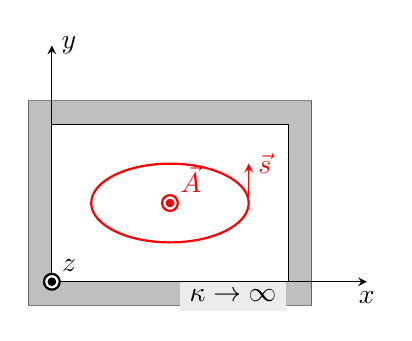
\begin{tikzpicture}
  \draw[fill=gray, opacity=0.5] (-0.3,-0.3) rectangle (3.3,2.3);
  \node[fill=lightgray!30] at (2.3,-0.18){$\kappa\to\infty$};
            \draw[thin, fill=white] (0,0) rectangle (3,2);
            \draw[thin,-stealth] (3,0) -- (4,0) node[below] {$x$}; 
            \draw[thin,-stealth] (0,2) -- (0,3) node[right] {$y$}; 
            \draw[fill=white, thick] (0,0) circle (0.1) node[anchor=south west]{$z$}; 
            \draw[fill=black, thick] (0,0) circle (0.04);
            \draw[red, thick] (1.5,1) circle (1 and 0.5);
            \draw[red, thin,-stealth] (2.5,1) -- +(0,0.5) node[right]{$\upd \vec{s}$};
            \draw[fill=white, thick, draw=red] (1.5,1) circle (0.1) node[anchor=south west,color=red]{$\upd \vec{A}$}; 
            \draw[fill=red, thick, draw=red] (1.5,1) circle (0.04);
          \end{tikzpicture}
          \end{column}
    \begin{column}{.65\textwidth}
  \begin{itemize}[<+->]
  \item Betrachte Ampèresches Durchflutungsgesetz \(\rotation\HFeld[v]=\StromDichte[v]+\frac{\d \DFeld[v]}{\d t}\) entlang einer beliebigen magnetischen Feldlinie:
    \begin{equation*}
      \oint_{O(A)} \BFeld[uv] \cdot \upd\vec{s} = \komplex\omega\varepsilon\mu \iint_{A} \EFeld[uv]\cdot\upd\vec{A} + \mu\iint_{A} \StromDichte[uv]\cdot\upd\vec{A}
    \end{equation*}
  \item \(\kappa\to\infty\): Feldlinie muss sich im Gebiet schließen
  \item Einfach zusammenhängend: Kein Strom durch Fläche
    \item Elektrisches Feld muss irgendwo z-Komponente haben oder Lösung ist die triviale Lösung.
  \end{itemize}
          \end{column}
\end{columns}    
\end{itemize}
\ 
\end{frame}

\begin{frame}
  \frametitle{TM- und TE-Lösungen}
  \begin{itemize}[<+->]
  \item Ausgangspunkt ist die \alert{Helmholtzgleichung} für \(\EFeld[uv]\):
    \begin{equation*}
      \laplace_t \EFeld[uv] + \left(\omega^2\varepsilon\mu -\Wellenzahl^2 \right) \EFeld[uv] = \laplace_t \EFeld[uv] + \gamma^2 \EFeld[uv] =  \vec{0}
    \end{equation*}
  \item Gleichungen für die Transversalkomponenten der Felder:
       \begin{align*}
      \EFeld[uv]_t &= \frac{\komplex}{\omega^2\varepsilon\mu - \Wellenzahl^2} \left[ \mp \Wellenzahl\, \gradient_t \EFeld[u]_{z} + \omega  \einheitsvek{z}\times\gradient_t \BFeld[u]_{z}\right]\\
      \BFeld[uv]_t &= \frac{\komplex}{\omega^2\varepsilon\mu - \Wellenzahl^2} \left[ \mp \Wellenzahl\, \gradient_t \BFeld[u]_{z} - \omega\varepsilon\mu  \einheitsvek{z}\times\gradient_t \EFeld[u]_{z}\right]
    \end{align*}

  \end{itemize}
\end{frame}


\begin{frame}
  \frametitle{TM-Lösungen -- \(\BFeld[u]_z = 0\)}
  \begin{itemize}[<+->]
  \item Betrachte \(z\)-Komponente der Helmholtzgleichung für \(\EFeld[uv]\):
    \begin{equation*}
      \boxed{\left(\laplace_t + \gamma^2\right) \EFeld[u]_z =  0} \text{ mit Randbedingung } \left. \EFeld[u]_z\right|_{O(V)} = 0 
    \end{equation*}
  \item Dieses \alert{Dirichletsche Randwertproblem} kann mit den Methoden der Elektrostatik gelöst werden. \(\to\) \alert{\(\EFeld[u]_z\) bekannt}
  \item Transversalkomponente des elektrischen Feldes für \(\BFeld[u]_z = 0\):
    \begin{equation*}
      \EFeld[uv]_t =  \mp \Wellenzahl \frac{\komplex}{\gamma^2} \, \gradient_t \EFeld[u]_{z}  \to \alert{\EFeld[uv]_t \text{ bekannt}}  
      \end{equation*}
  \item Transversalkomponente der magnetischen Flussdichte für \(\BFeld[u]_z = 0\):
       \begin{align*}
         \BFeld[uv]_t = \mu\HFeld[uv]_t&= -\frac{\komplex}{\gamma^2} \omega\varepsilon\mu  \einheitsvek{z}\times\gradient_t \EFeld[u]_{z}\\
         &= \pm \frac{\omega\varepsilon\mu}{\Wellenzahl} \einheitsvek{z}\times \EFeld[uv]_{t} = \pm \mu \frac{1}{Z} \einheitsvek{z}\times \EFeld[uv]_{t} \text{ mit } Z=\frac{\Wellenzahl}{\omega\varepsilon} = \frac{\Wellenzahl}{\Wellenzahl_0}\sqrt{\frac{\mu}{\varepsilon}} = \frac{\Wellenzahl}{\Wellenzahl_0} Z_0 
       \end{align*}
       \item Damit ist auch die \alert{magnetische Flussdichte im Lösungsvolumen bestimmt}. 
       \end{itemize}
       \ 
\end{frame}


\begin{frame}
  \frametitle{TE-Lösungen -- \(\EFeld[u]_z = 0\)}
  \begin{itemize}[<+->]
  \item Betrachte \(z\)-Komponente der Helmholtzgleichung für \(\HFeld[uv]\):
    \begin{equation*}
      \boxed{\left(\laplace_t + \gamma^2\right) \HFeld[u]_z =  0} \text{ mit Randbedingung } \left. \frac{\d \HFeld[u]_z}{\d \vec{n}}\right|_{O(V)} = 0 
    \end{equation*}
  \item Dieses \alert{Neumannsche Randwertproblem} kann mit den Methoden der Magnetostatik gelöst werden. \(\to\) \alert{\(\HFeld[u]_z\) bekannt}
  \item Transversalkomponente des magnetischen Feldes für \(\EFeld[u]_z = 0\):
    \begin{equation*}
      \HFeld[uv]_t = \mp \frac{\komplex}{\gamma^2} \Wellenzahl\, \gradient_t \HFeld[u]_{z}  \to \alert{\HFeld[uv]_t \text{ bekannt}}
    \end{equation*}
  \item Transversalkomponente der elektrischen Feldes für \(\EFeld[u]_z = 0\):
       \begin{align*}
         \EFeld[uv]_t &= \pm Z\, \einheitsvek{z}\times \HFeld[uv]_{t} \text{ mit } Z=\frac{\mu\omega}{\Wellenzahl} = \frac{\Wellenzahl_0}{\Wellenzahl}\sqrt{\frac{\mu}{\varepsilon}} = \frac{\Wellenzahl_0}{\Wellenzahl} Z_0 
       \end{align*}
       \item Damit ist auch die \alert{elektrische Feldstärke im Lösungsvolumen bestimmt}. 
       \end{itemize}
       \ 
\end{frame}


\begin{frame}
  \frametitle{Diskussion der TM- und TE-Lösungen}
  \begin{itemize}[<+->]
  \item Für den \alert{TEM-Mode} hatten wir schon gesehen, dass für ihn -- wenn er existiert -- die \alert{Dispersionsrelation des TEM-Modes} erfüllt sein muss:
    \begin{equation*}
      \gamma^2=0 \Leftrightarrow \boxed{\Wellenzahl=\Wellenzahl_0=\omega\sqrt{\varepsilon\mu}}
    \end{equation*}
  \item Wenn der TEM-Mode existiert, existiert es für beliebige Frequenzen!
  \item Das ist bei TM- und TE-moden anders! Z.B. für den TM-Mode muss zunächst das Randwertproblem zur \(\EFeld[u]_z\) gelöst werden:
    \begin{equation*}
      \left(\laplace_t + \gamma^2\right) \EFeld[u]_z =  0 \text{ mit } \left. \EFeld[u]_z\right|_{O(V)} = 0
    \end{equation*}
  \item Dies ist eine \alert{Eigenwertgleichung} für die \alert{Eigenfunktionen=Moden} \(\EFeld[u]_{z\lambda}\) und den (diskreten) \alert{Eigenwerten} \(\gamma^2_\lambda\) mit \(\lambda = 1,2,3,\ldots\).
   \begin{equation*}
      \left(\laplace_t + \gamma_\lambda^2\right) \EFeld[u]_{z\lambda} =  0
    \end{equation*}
  \item Für eine Kreisfrequenz \(\omega\) gilt dann
    \begin{equation*}
      \gamma_\lambda^2 = \mu\varepsilon\omega^2-\Wellenzahl_\lambda^2 \Rightarrow \Wellenzahl_\lambda=\sqrt{\mu\varepsilon\omega^2-\gamma^2} \Rightarrow  \boxed{\Wellenzahl_\lambda=\sqrt{\mu\varepsilon}\sqrt{\omega^2-\omega_\lambda^2}} \text{ mit } \omega_\lambda=\frac{\gamma_\lambda}{\sqrt{\mu\varepsilon}} 
      \end{equation*}
 \end{itemize}
\end{frame}

\begin{frame}
  \frametitle{Cut-Off -- Evaneszente Moden}
  \begin{itemize}[<+->]
  \item Wir haben die \alert{Dispersionsrelation}
    \begin{equation*}
      \Wellenzahl_\lambda=\sqrt{\mu\varepsilon}\sqrt{\omega^2-\omega_\lambda^2} \text{ mit } \omega_\lambda=\frac{\gamma_\lambda}{\sqrt{\mu\varepsilon}} 
    \end{equation*}
  \item Die \(z\)-Abhängigkeit der Lösung ist (z.B. für das elektrische Feld)
             \begin{equation*}
           \EFeld[uv]_\lambda(\Ortsr[v]) = \EFeld[uv]_{0\lambda}(x,y) \euler^{\pm\komplex\Wellenzahl_\lambda z}
         \end{equation*}
   \item Für \alert{\(\omega < \omega_\lambda\)} wird \(\Wellenzahl_\lambda\) \alert{imaginär} und die Lösung ist \alert{keine propagierende Welle} mehr. Diese Lösungen sind \alert{evaneszente Moden}:
\begin{equation*}
           \EFeld[uv]_\lambda(\Ortsr[v]) = \EFeld[uv]_{0\lambda}(x,y) \euler^{\mp|\Wellenzahl_\lambda| z} \text{ für } \omega < \omega_\lambda
         \end{equation*}
         \item Die (Kreis)-Frequenz \(\omega_\lambda = 2\pi f_\lambda\) heißt \alert{Cut-Off Frequenz} des Modes \(\lambda\). 
 \end{itemize}
\end{frame}

\begin{frame}
  \frametitle{Dispersionsrelation}
  \begin{itemize}[<+->]
  \item Wir können die Dispersionsrelation \(\Wellenzahl_\lambda=\sqrt{\mu\varepsilon}\sqrt{\omega^2-\omega_\lambda^2}\) auf \(\Wellenzahl_0=\sqrt{\mu\varepsilon}\omega\) normieren:
    \begin{equation*}
      \frac{\Wellenzahl_\lambda}{\Wellenzahl_0}=\sqrt{1-\frac{\omega_\lambda^2}{\omega^2}}
    \end{equation*}
  \item Dies ergibt folgendes Bild:
    \bigskip
    
    \begin{tikzpicture}[scale=1]
      \begin{axis}[
        grid=both,
        xmin = 0, xmax = 6,
        ymin = 0, ymax = 1.2,
        xtick = {0,1,2,4,4.5,5},
        xlabel = {$\omega$},
        ylabel = {$\frac{\Wellenzahl_\lambda}{\Wellenzahl}$},
        xticklabels = {0, $\omega_1$, $\omega_2$, $\omega_3$, $\omega_4$, $\omega_5$},
        width=\textwidth,height=.65\textheight]
        \addplot[domain=0:6,samples=500,smooth,thick,red] {sqrt(1.-(1./x)^2)}; 
        \addplot[domain=0:6,samples=500,smooth,thick,green] {sqrt(1.-(2./x)^2)};         
        \addplot[domain=0:6,samples=500,smooth,thick,blue] {sqrt(1.-(4./x)^2)}; 
        \addplot[domain=0:6,samples=500,smooth,thick,cyan] {sqrt(1.-(4.5/x)^2)}; 
        \addplot[domain=0:6,samples=500,smooth,thick,magenta] {sqrt(1.-(5./x)^2)}; 
        \addplot[domain=0:6,samples=100,smooth,thick,black] {1} [yshift=8pt] node[pos=0.35] {TEM-Mode (falls nicht einfach zusammenhängend)};
        \node [color=green] at (3,0.1) {2 Moden (+TEM)};
    \end{axis}
\end{tikzpicture}    
\end{itemize}
\ 
\end{frame}

\begin{frame}
  \frametitle{Phasen- und Gruppengeschwindigkeiten}
  \begin{itemize}[<+->]
  \item \alert{Phasengeschwindigkeit} ist definiert als \(\Geschwindigkeit_p = \frac{\omega}{\Wellenzahl}\)
    \begin{itemize}[<+->]
    \item TEM-Mode \(\Wellenzahl_0=\sqrt{\varepsilon\mu}\, \omega\): 
      \begin{equation*}
        \Geschwindigkeit_{p0} = \frac{\omega}{\Wellenzahl_0} = \frac{1}{\sqrt{\varepsilon\mu}} = \Geschwindigkeit_c
        \end{equation*}
      \item TM/TE-Mode \(\Wellenzahl_\lambda=\sqrt{\mu\varepsilon}\sqrt{\omega^2-\omega_\lambda^2}\):
      \begin{equation*}
        \Geschwindigkeit_{p\lambda} = \frac{\omega}{\Wellenzahl_\lambda} = \frac{\Geschwindigkeit_{p0}}{\sqrt{1-\frac{\omega_\lambda^2}{\omega^2}}} = \frac{\Geschwindigkeit_{c}}{\sqrt{1-\frac{\omega_\lambda^2}{\omega^2}}}\quad \Geschwindigkeit_{p\lambda}(\omega\to\omega_\lambda)\to\infty \quad \Geschwindigkeit_{p\lambda}(\omega\to\infty)\to\Geschwindigkeit_c 
        \end{equation*}
        
  \end{itemize}
  \item \alert{Gruppengeschwindigkeit} ist definiert als \(\Geschwindigkeit_g = \frac{\d \omega}{\d \Wellenzahl}\)
    \begin{itemize}[<+->]
    \item TEM-Mode \(\Wellenzahl_0=\sqrt{\varepsilon\mu}\, \omega\): 
      \begin{equation*}
        \Geschwindigkeit_{g0} = \frac{\omega}{\Wellenzahl_0} = \frac{1}{\sqrt{\varepsilon\mu}} = \Geschwindigkeit_{p0}=\Geschwindigkeit_c
        \end{equation*}
      \item TM/TE-Mode \(\Wellenzahl_\lambda=\sqrt{\mu\varepsilon}\sqrt{\omega^2-\omega_\lambda^2}\):
      \begin{equation*}
        \Geschwindigkeit_{g\lambda} = \frac{\d \omega}{\d \Wellenzahl_\lambda} = \Geschwindigkeit_{c} \sqrt{1-\frac{\omega_\lambda^2}{\omega^2}} \quad \Geschwindigkeit_{g\lambda}(\omega\to\omega_\lambda)=0 \quad \Geschwindigkeit_{g\lambda}(\omega\to\infty)\to\Geschwindigkeit_c 
        \end{equation*}
        
  \end{itemize}
  \end{itemize}
\end{frame}


\begin{frame}
  \frametitle{Modenentartung}
  \begin{itemize}[<+->]
  \item Gerade bei Querschnitten mit \alert{hoher Symmetrie} (z.B. quadratischer Querschnitt) kommt es dazu, \alert{Eigenwerte übereinstimmen}.
  \item Man spricht in diesem Fall von \alert{Entartung}.
  \item In diesem Fall ergeben sich verschiedene \alert{Eigenfunktionen} (Moden) zu identischen Grenzfrequenzen \(\omega_{\lambda_1} = \omega_{\lambda_2}\)
  \item Gibt es \(n\) Eigenlösungen zu einem Eigenwert spricht man von einer \alert{\(n\)-fachen Entartung}
    \item Technisch ist es sehr häufig erwünscht, nur einen ausbreitungsfähigen Mode im Arbeitsbereich zu haben (\alert{Single-Mode-Betrieb}) 
  \end{itemize}
\end{frame}
    
\input{finalframe.inc}
   
\end{document}